

\subsection{Project Timeline}
This is a very important component in every project in order to achieve goals, aims and objectives of this project, the project is divided into two parts the program development and project documentation. The program development is sub-divided into three parts; client, core, services and documentation. The project documentation contains the following; introduction, review, requirement and design, implementation, teamwork, evaluation and peer assessment. Below is the time plan:
\begin{center}
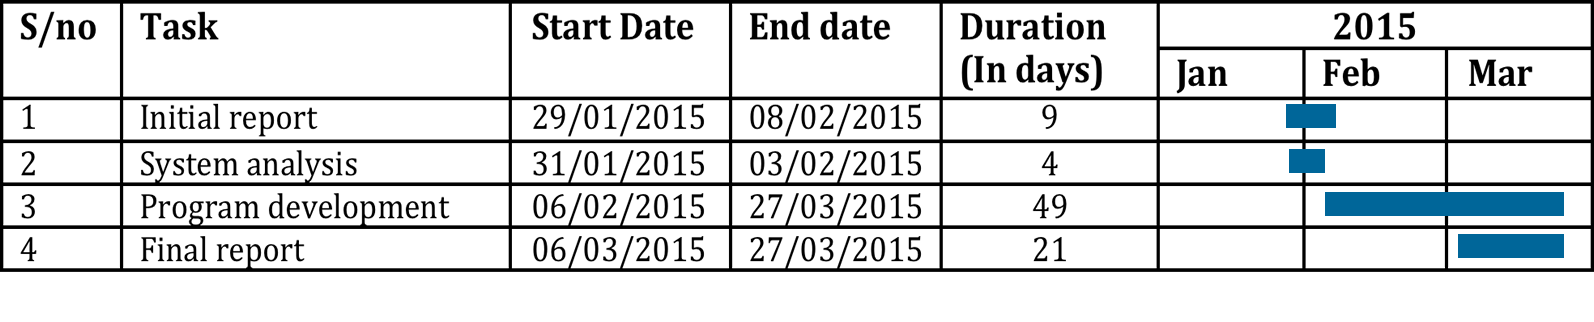
\includegraphics[scale=0.8]{./images/ganttchart.png}
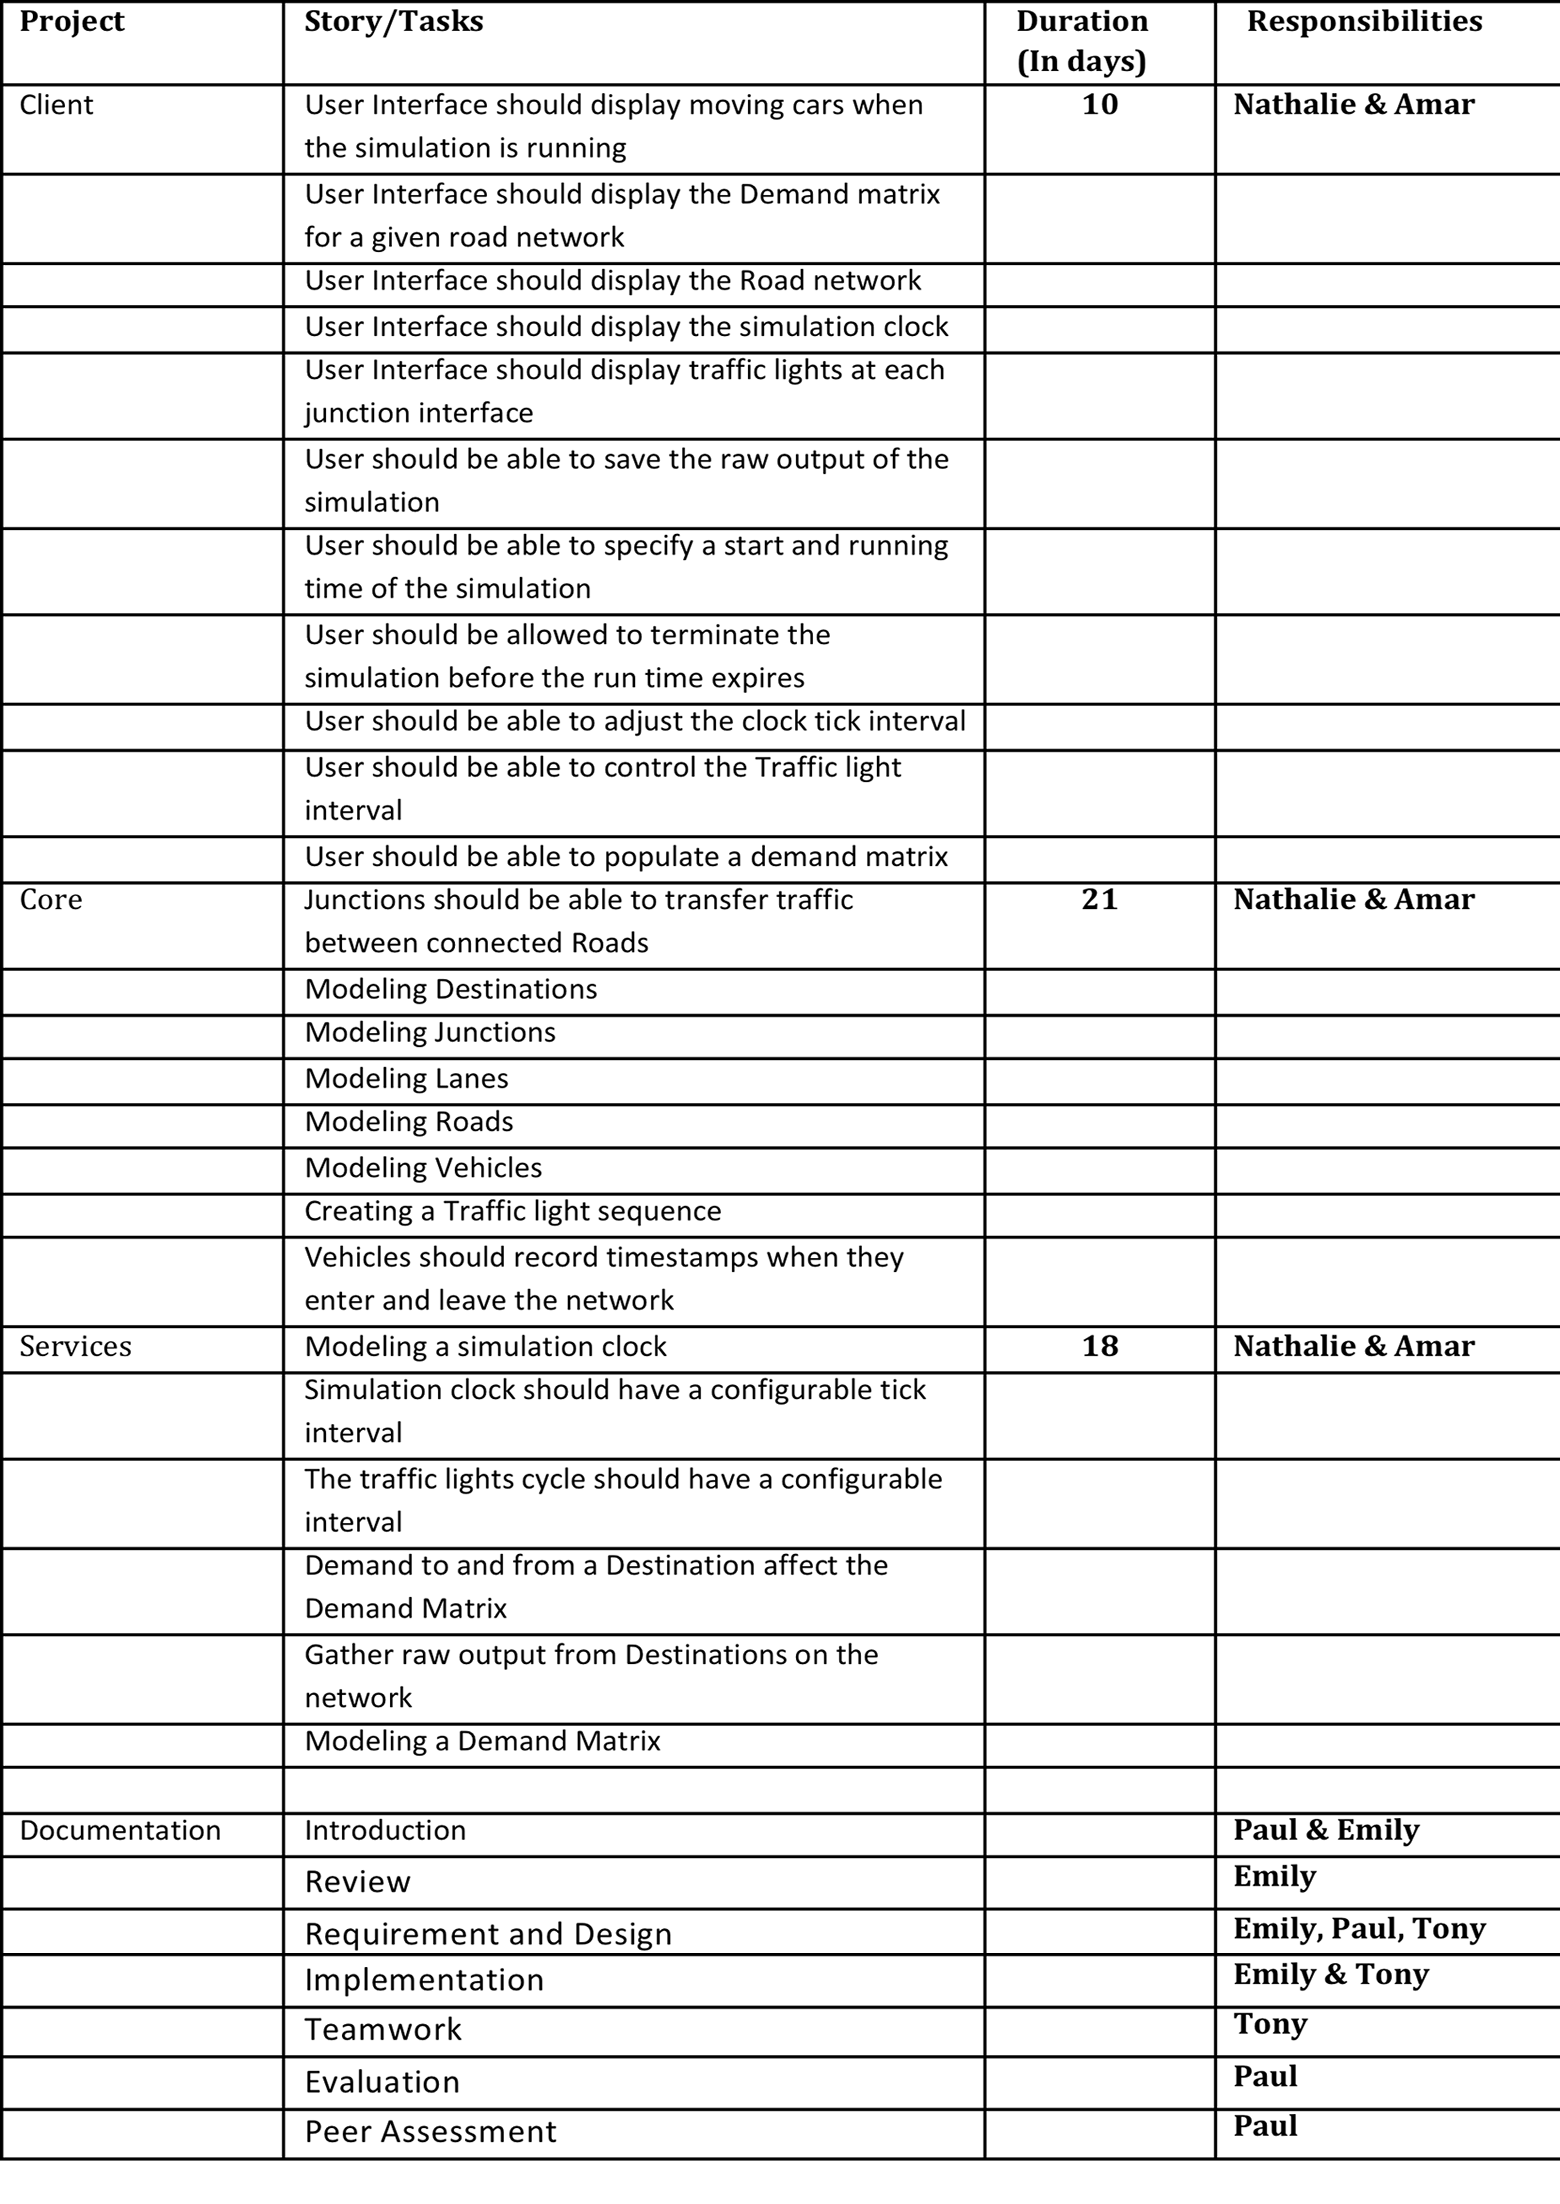
\includegraphics[scale=0.6]{./images/schedule.png}
\end{center}

\subsection{UI Design and Implementation}
We implemented the system using Java because that is the language that the majority of the team was most familiar with. We also wrote a small script in python to summarise the output.

One of the main objectives of the Traffic Simulator project was for it to have an interactive UI. There were a couple of vital reasons for designing the UI as we did. Firstly the project were based in Java so you could understand the code and see a large portion of how it worked. Also from a another perspective the simulation of the traffic network with different roads, lanes and vehicles allows the traffic analyst or developer to view a considerable measure of the core of what was going on and that is something that we sought in our project too.

\begin{center}
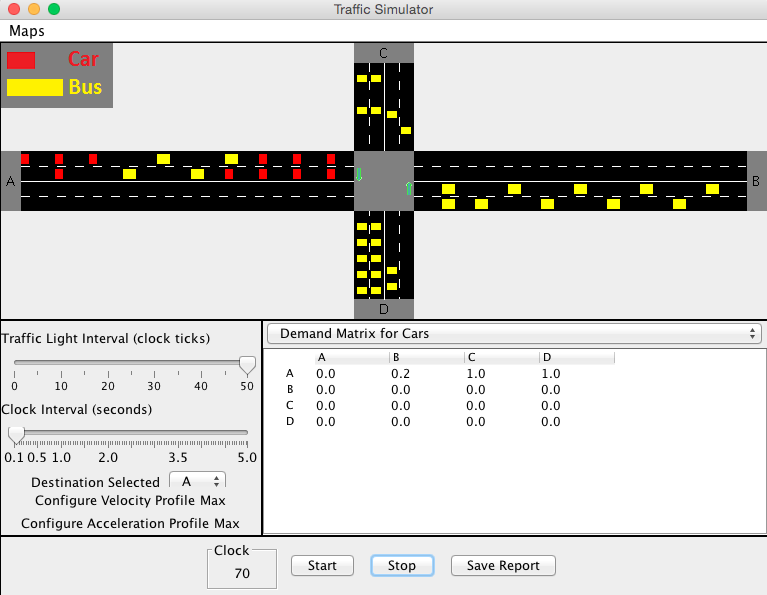
\includegraphics[scale=0.4]{./images/network1.png}
\end{center}


\subsection{Output}
We designed the software to output individual car journeys for a transport consultant to analyse using statistical analysis packages.  The basic idea is that the software is used to support decisions about  changes to the road network or for supporting planning decisions.  We present two scenarios here. Instead of using a statistical analysis package such as SPSS we wrote a custom python script to summarise the data.  The script also serves as a sanity check for the output of our software.  The python script is included in the appendix to this report. 



\subsubsection{Shopping Centre Development}
We have a simple network as shown below.  The consultant does a survey to measure existing traffic movements which we translate into a \textit{demand matrix} for the road system.  The demand matrix is just a count of car movements between each end point of the network over a given time period.  We are keeping things simple in our example and only considering one vehicle type.  In reality the model would take into account of other vehicle types and our software does allow for that.  We convert this demand matrix into a table which specifies the probability of a car entering the network at for each combination of origin and destination for each tick of the simulation clock.  This drives the creation of vehicles in our simulation for the base case.  \\ The consultant runs other models, based on the size of the new shopping centre and proximity of other centres to estimate a new demand matrix for when the centre is built.  Our software is then run in the base case and the modelled case using the new demand matrix and reports are generated showing the effect on journey times.\\  \newpage \textbf{Network diagram}\\
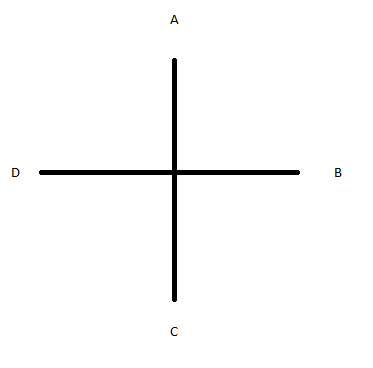
\includegraphics[scale=0.5]{./images/network.png}

We used the following trip matrix for the base case:
	\begin{center}
	\begin{tabular}{| c | c | c | c | c |}
		\hline
		\textbf{ }	&	A & B & C & D \\ \hline
		A				&	0 & 0.3 & 0.3 & 0.3				\\ \hline
		B					&	0.3 & 0 & 0.3 & 0.3				\\ \hline
		C	&	0.3 & 0.3 & 0 & 0.3			\\ \hline
		D				&	0.3 & 0.3 & 0.3 & 0				\\ \hline

		
	\end{tabular}
	\end{center} and the following matrix, showing extra demand to and from the shopping centre at C
    \begin{center}
	\begin{tabular}{| c | c | c | c | c |}
		\hline
		\textbf{ }	&	A & B & C & D \\ \hline
		A				&	0 & 0.3 & 0.8 & 0.3				\\ \hline
		B					&	0.3 & 0 & 0.8 & 0.3				\\ \hline
		C	&	0.5 & 0.5 & 0 & 0.5			\\ \hline
		D				&	0.3 & 0.3 & 0.8 & 0				\\ \hline

		
	\end{tabular}
	\end{center}
    
    The output supports the case for the shopping centre  proportionally more cars going to and from C but the average journey times overall have not increased, although journeys to the shopping centre inself have slowed. This shows that the road network can support extra traffic without significant problems except around the centre itself.  The output for the two cases is shown below\\ \newpage \textbf{Base case}\\
    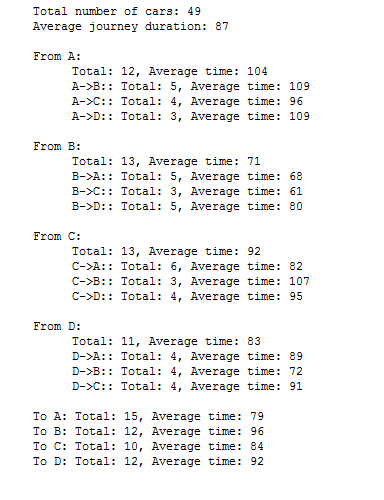
\includegraphics[scale=0.8]{./images/scenario1.png}\\ \newpage \textbf{Planned Shopping Centre}\\
    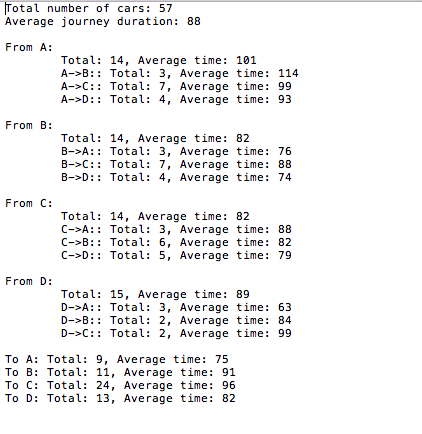
\includegraphics[scale=0.8]{./images/scenario2_1.png}
    
    
\subsubsection{Congestion Charge}
This scenario is similar to the Shopping Centre example but this time we are reducing demand for journeys to one node in the network by introducing a toll in the road system.  We should see a reduction in journey times as congestion is reduced.
   
    

In this case we used the following trip matrix and got the output below, which supports the case for a congestion charge at C reducing journey times
 \begin{center}
	\begin{tabular}{| c | c | c | c | c |}
		\hline
		\textbf{ }	&	A & B & C & D \\ \hline
		A				&	0 & 0.5 & 0.1 & 0.3				\\ \hline
		B					&	0.3 & 0 & 0.1 & 0.3				\\ \hline
		C	&	0.3 & 0.3 & 0 & 0.3			\\ \hline
		D				&	0.3 & 0.5 & 0.1 & 0				\\ \hline

		
	\end{tabular}
	\end{center}
~ \\ \textbf{Congestion charge}\\
    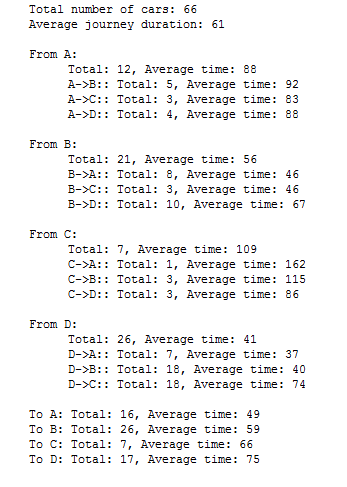
\includegraphics[scale=1.0]{./images/scenario3.png}